%!TEX root = ../dissertation.tex
\begin{savequote}[75mm]
Nulla facilisi. In vel sem. Morbi id urna in diam dignissim feugiat. Proin molestie tortor eu velit. Aliquam erat volutpat. Nullam ultrices, diam tempus vulputate egestas, eros pede varius leo.
\qauthor{Quoteauthor Lastname}
\end{savequote}

\chapter{Related works}

\section{Phrase Grounding}

Phrase grounding is the task that studies the mapping from noun
phrases to regions of an image (Sec.~\ref{sec:visual-grounding}) and
requires strong understanding of both visual and textual modalities,
specially when not all ground truth is available. 

Even if phrase groudning is an extremely relevant task, the study of
this problem in literature starts relatively late, mostly because a
community-accepted formalization of the problem took its time for
being developed. First efforts in this direction can be identified by
the work of S. Fidler \etal{} \cite{fidler2013sentence}. They
developed a model for semantic understanding of scene exploiting both
textual and visual information. In their work, short sentences are
parsed into nouns and prepositions, which are used to generate
potentials in a holistic scene model. An attempt to find an alignment
between entities in image and sentence is done by C. Kont \etal{}
\cite{kong2014you}. They proposed a model that exploits potentials
computed from text and RGB-D imagery to reason about the class of the
3D objects, the scene type, as well as to align the nouns/pronouns
with the referred visual objects. They used complex sentences, but
grounding is contrained to nouns of 21 object classes relevant to
indoor scenes. In the same period, R. Hu \etal{} \cite{hu2016natural}
moved to a sligtly different task that requires to localize a target
object within a given image based on a natural language query of the
object, named natural language object retrieval. It differs from
text-based image retrieval task as it involves spatial information
about objects within the scene and global scene context. To address
this issue, they proposed a novel Spatial Context Recurrent ConvNet
(SCRC) model as scoring function on candidate boxes for object
retrieval, integrating spatial configurations and global scene-level
contextual information into the network. In particular, their model
processes query text, local image descriptors, spatial configurations
and global context features through a recurrent network, outputs the
probability of the query text conditioned on each candidate box as a
score for the box, and can transfer visual-linguistic knowledge from
image captioning domain to their task. The advent of Flickr30k
Entities dataset collected and processed by B. Plummer \etal{}
\cite{plummer2015flickr30k} (described in Sec.~\ref{subsec:flickr30k})
boosted the development of morea accurate and general models, and
allowed to face the problem phrase grounding without constraints.
Along with the new dataset, they also provided a strong baseline for
phrase grounding based on Canonical Correlation Analysis (CCA) for
phrase grounding task. Their baseline consists in scoring each
region-phrase correspondence separately, without taking into accont
any context of performing any joint inference about the global
correspondence between all regions in the image and all phrases in the
sentence. On the countrary, L. Wang \etal{} in \cite{wang2016learning}
proposed a method for learning joint embeddings of images and text
using a two-branch neural network with multiple layers of linear
projections followed by nonlinearities. The network is trained using a
large margin objective that combines cross-view ranking constraints
with within-view neighborhood structure preservation constraints
inspired by metric learning literature. In
\cite{rohrbach2016grounding}, A. Rohrbach \etal{}, authors developed a
model able to reconstruct textual features in an encoder-decoder
fashion, powered by an attention module which implements localization
of regions of interest. Here, the attention is used to both ground and
reconstruct. During training, the attention learns how to reconstruct
given sentence describing the region to ground. During inference,
attention localizes such region. The key motivation under this idea is
that by training to reconstruct the text phrase, the model learn first
to ground the phrase in the image. Moreover, their model is able to
work with no, semi or full supervision. When no ground truth is
available, the model simply learns to reconstruct the given sentence.
Otherwise, the correct localization is enforced besides the
reconstruction.

As A. Rohrbach \etal{} proved \cite{rohrbach2016grounding}, phrase
grounding problem can be addressed even with some or no ground truth,
allowing, on one side, to learn a more natural approach for grounding,
i.e., wihtout memorizing mapping from phrases to boxes and, on the
other side, to reduce the expansive annotations required with full
supervision. Those annotation, as primarily pointed out by Flickr30k
Entities authors \cite{plummer2015flickr30k} requires a good amount of
work (implying time and money) to be collected because the need of
manual annotators. Large corpus of text and images instead were
already available. Otherwise, even the collection of a new dataset
with shallow information like the link between an image and its
caption is relatively easy to collect. On this wave, many researches
tried to tackle phrase grounding in weak supervised settings.  For
example, F. Xiao \etal{} in \cite{xiao2017weakly} proposed a a
weakly-supervised approach that takes image-sentence pairs as input
and learns to visually ground arbitrary linguistic phrases, in the
form of spatial attention masks. To this end, they introduce an
end-to-end model which learns visual groundings of phrases with two
types of loss functions. In addition to the standard discriminative
loss, which enforces that attended image regions and phrases are
consistently encoded, they propose a novel structural loss which makes
use of the parse tree structures induced by the sentences. In
particular, they ensure complementarity among the attention masks that
correspond to sibling noun phrases, and compositionality of attention
masks among the children and parent phrases, as defined by the
sentence parse tree. Technically speaking, their model encodes a
sentence through a two-layers RNN with LSTM cells and a Dropout model
to prevent overfitting, obtaining $\phi_L(P)$ the language code. The
visual code $\phi_V(I)$ is computed insted by an embedding module,
i.e., a two-layer perceptron with Dropout, that projects features from
VGG-16 convolutional layers to a latent space. Leveragin on weak
annotations their discriminative loss enforces the codes to be similar
when features belongs to linked examples, otherwise to be different.
Formally, given $I_i$ an image and $\{ P^1_i, P^2_i, \ldots, P^n_i \}$
a set of corresponging phrases (both positive and negative), 
\begin{equation}
  L_{disc} = -Y^j_i \cdot Sigmoid(\phi_V(I_i) \cdot \phi_L(P^j_i))
\end{equation}
where $Y^j_i \in \{ -1, +1 \}$ is the indicator variable denoting
whether $P^j_i$ s a negative/positive match to $I_i$. The structural
loss instead heavily exploit relations on sentence structure to
generate an attention mask for localization. A parser first extract
parent-sibling (PC) and sibling-sibling (SIB) relation. Such
constraints are then enforced on the attention mask throught the two
structural loss components $L_{PC}$ and $L_{SIB}$. $L_{PC}$, defined
as 
\begin{equation}
  L_{PC} = \frac{1}{|P|} \sum_{k \in P} \mid A_k - \max_{l \in child(k)} A_l \mid ^ 2,
\end{equation}
tries to bring the attention mask of a parent node and the union mask
of all its children nodes to be close to one another, while
\begin{equation}
  L_{SIB} = - \frac{1}{|S|} \sum_{m \in S} \sum_{pixels \in A} W_m \cdot \log \frac{\max_n A_{m,n}}{\sum_n A_{m,n}}
\end{equation}
introduces competition such that the attention masks of sibling nodes
are exclusive for every pixel.

A few months later, following the idea of attention mask, H. Akbari
\etal{} in \cite{akbari2019multi} addressed the problem of phrase
localization  by learning a multi-level common semantic space shared
by the textual and visual modalities. We exploit multiple levels of
feature maps of a Deep Convolutional Neural Network, as well as
contextualized word and sentence embeddings extracted from a
character-based language model. Following dedicated non-linear
mappings for visual features at each level, word, and sentence
embeddings, we obtain multiple instantiations of our common semantic
space in which comparisons between any target text and the visual
content is performed with cosine similarity. We guide the model by a
multi-level multimodal attention mechanism which outputs attended
visual features at each level. The best level is chosen to be compared
with text content for maximizing the pertinence scores of
image-sentence pairs of the ground truth.

S. A. Javed \etal{} in \cite{javed2018learning} proposed a different
and interesting approach by learning to ground thought a proxy task.
They propose a novel framework for unsupervised visual grounding which
uses concept learning to obtain self-supervision. The intuition behind
this idea is to encourage the model to localize to regions which can
explain some semantic property in the data, such us, the property
being the presence of a concept in a set of images. Basically, given a
set of pairs image and caption all belonging to the same concept, the
model must decode the common concept in the batch. Their model follows
a typical encoder-decoder architecture where the encoder localizes the
region that represents the batch's concept as an heatmap, while
decoder reconstruct the common concept throuhgt a classifier. The
concept batch is constructed by grouping together $k$ pairs image,
caption where all captions contains the same concept. Concept is
extracted from a phrase by selecting all nouns in a phrase thought a
POS tagger and randomly picking one of them.

The idea of using a form of external knowledge is taken up by K. Chen
\etal{} in \cite{chen2018knowledge}, where they approached the problem
by learning to reconstruct the input. However, their approach is
slightly different wrt similar works where the optimization is solely
guided by the reconstruction loss from the language modality. Instead,
it encompasses rich visual information contained in proposals and
useful cues from external knowledge. Their major contributions are
twofold. In order to attend relevant features they introduce the
knowledge base pooling (KBP) gate which returns a score between query
and proposal content computed on the word embedding of proposal
classification label. Basically, they leverage the pretrained object
detector which, along with the proposal, returns a probability
distribution on a vocabulary of labels, used to semantically
categorize the content of the proposal. Such score is computed with a
similarity function (like the cosine similarity) between the word
embeddings of a representative word in query and the proposal class
label. The query representative is computed by averaging the
embeddings of all nouns in the query. Then, they reconstruct both
visual and language modalities. The visual modality is reconstructed
by an attention module that takes embedded features and predicts new
proposal coordinates by optimizing them to be as close as possible to
proposal's. Predicted coordinates as multiplied by the computed
knowledge by KBP gate. The goal of visual consistency branch is to
optimize the attention model via learning to predict location
information contained in query-related proposals. The language
modality is instead reconstructed in a classical way by predicting
thought an RNN with LSTM cells. An high-level overview of the model is
shown in Fig.~\ref{fig:kac-example}.

\begin{figure}
  \centering
  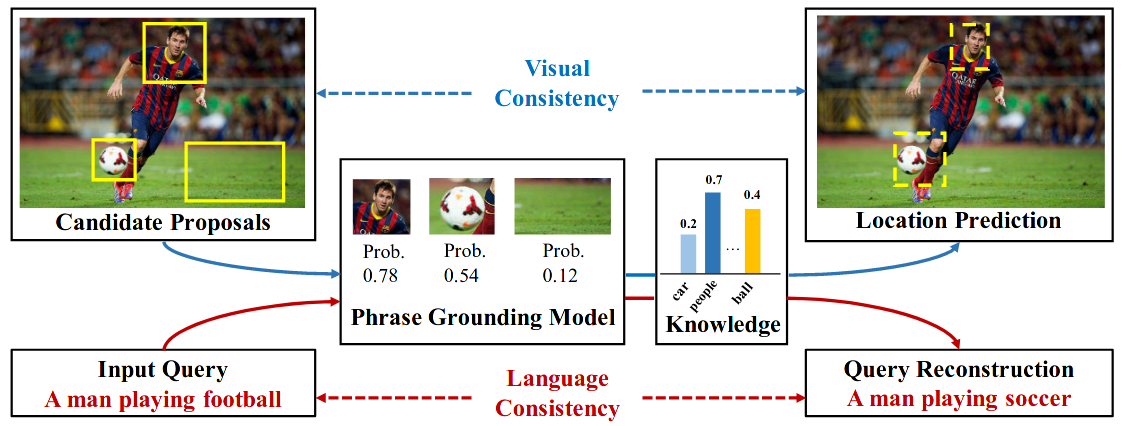
\includegraphics[width=.8\textwidth]{figures/kac-example.png}
  \caption[Knowledge Aided Consistency high-level architecture
  overview]{Knowledge Aided Consistency high-level architecture
  overview \cite{chen2018knowledge}. KAC Net applies both visual and
  language consistency and leverages complementary knowledge from
  the visual feature extractor to facilitate weakly supervised
  grounding.}
  \label{fig:kac-example}
\end{figure}

In \cite{liu2019adaptive}, X. Liu \etal{} proposed a reconstruction
network based on attention map and optimized for the task of REG
(Sec.~\ref{sec:visual-grounding}). They extract the subject, location
and context features to represent the proposals and the query
respectively. Then, they design the adaptive grounding module to
compute the matching score between each proposal and query by a
hierarchical attention model. Finally, based on attention score and
proposal features, they reconstruct the input query with a
collaborative loss of language reconstruction loss, adaptive
reconstruction loss, and attribute classification loss. The key idea
under their approach is that this adaptive mechanism helps alleviating
the variance of different referring expressions.

S. Datta \textit{et al.} in \cite{datta2019align2ground} proposed a
system able to learn phrase grounding by optimizing the model for the
downstream task of caption-to-image retrieval. Their key contribution
lies in building a sort of caption-conditioned image encoding which
tightly couples both the tasks and allows the weak supervision to
effectively guide visual grounding. Their method is composed by three
modules. As a first step, it infers the latent correspondences between
regions-of-interest (RoIs) and phrases in the caption and creates a
discriminative image representation using these matched RoIs.
Practically, they project both visual and textual features in a joint
embedding space by linear projection. Then, using a similarity
function, they compute the similarity between each phrase and each
RoI. For each phrase, the module returns a random proposal among top-k
($k = 3$) similar proposals wrt the phrase. The intention here is to produce a list of caption-conditioned RoIs. In the second step, they build a global representation of previously matched RoIs with an order-invariant deep encoder. The encoder is imlemented as a two-layer MLP. Finally, they measure the similarity between the proposed image representation and the
query caption by first embeddings the caption $c$, encoded
by $\Phi_{RNN}$, in the same output space as the image representation  $I^c_{rois}$ by using a two-layer MLP $f_{enc}$:
\begin{equation}
  \hat{\bm{c}} = MLP (\Phi_{RNN} (c)) \qquad \hat{\bm{r}}_c = f_{enc} (I^c_{rois}).
\end{equation}
We then compute cosine
similarity between the two multimodal representations.
\begin{equation}
  S_{Ic} = \frac{ \hat{\bm{c}}^T \hat{\bm{r}}_c }{ || \hat{\bm{c}} ||_2 || \hat{\bm{r}}_c ||_2 }.
\end{equation}
where $S_{Ic}$ is the similarity between image $I$ and caption $c$. Thei model overview is shown in Fig.~\ref{fig:align2ground-model}.

\begin{figure}
  \centering
  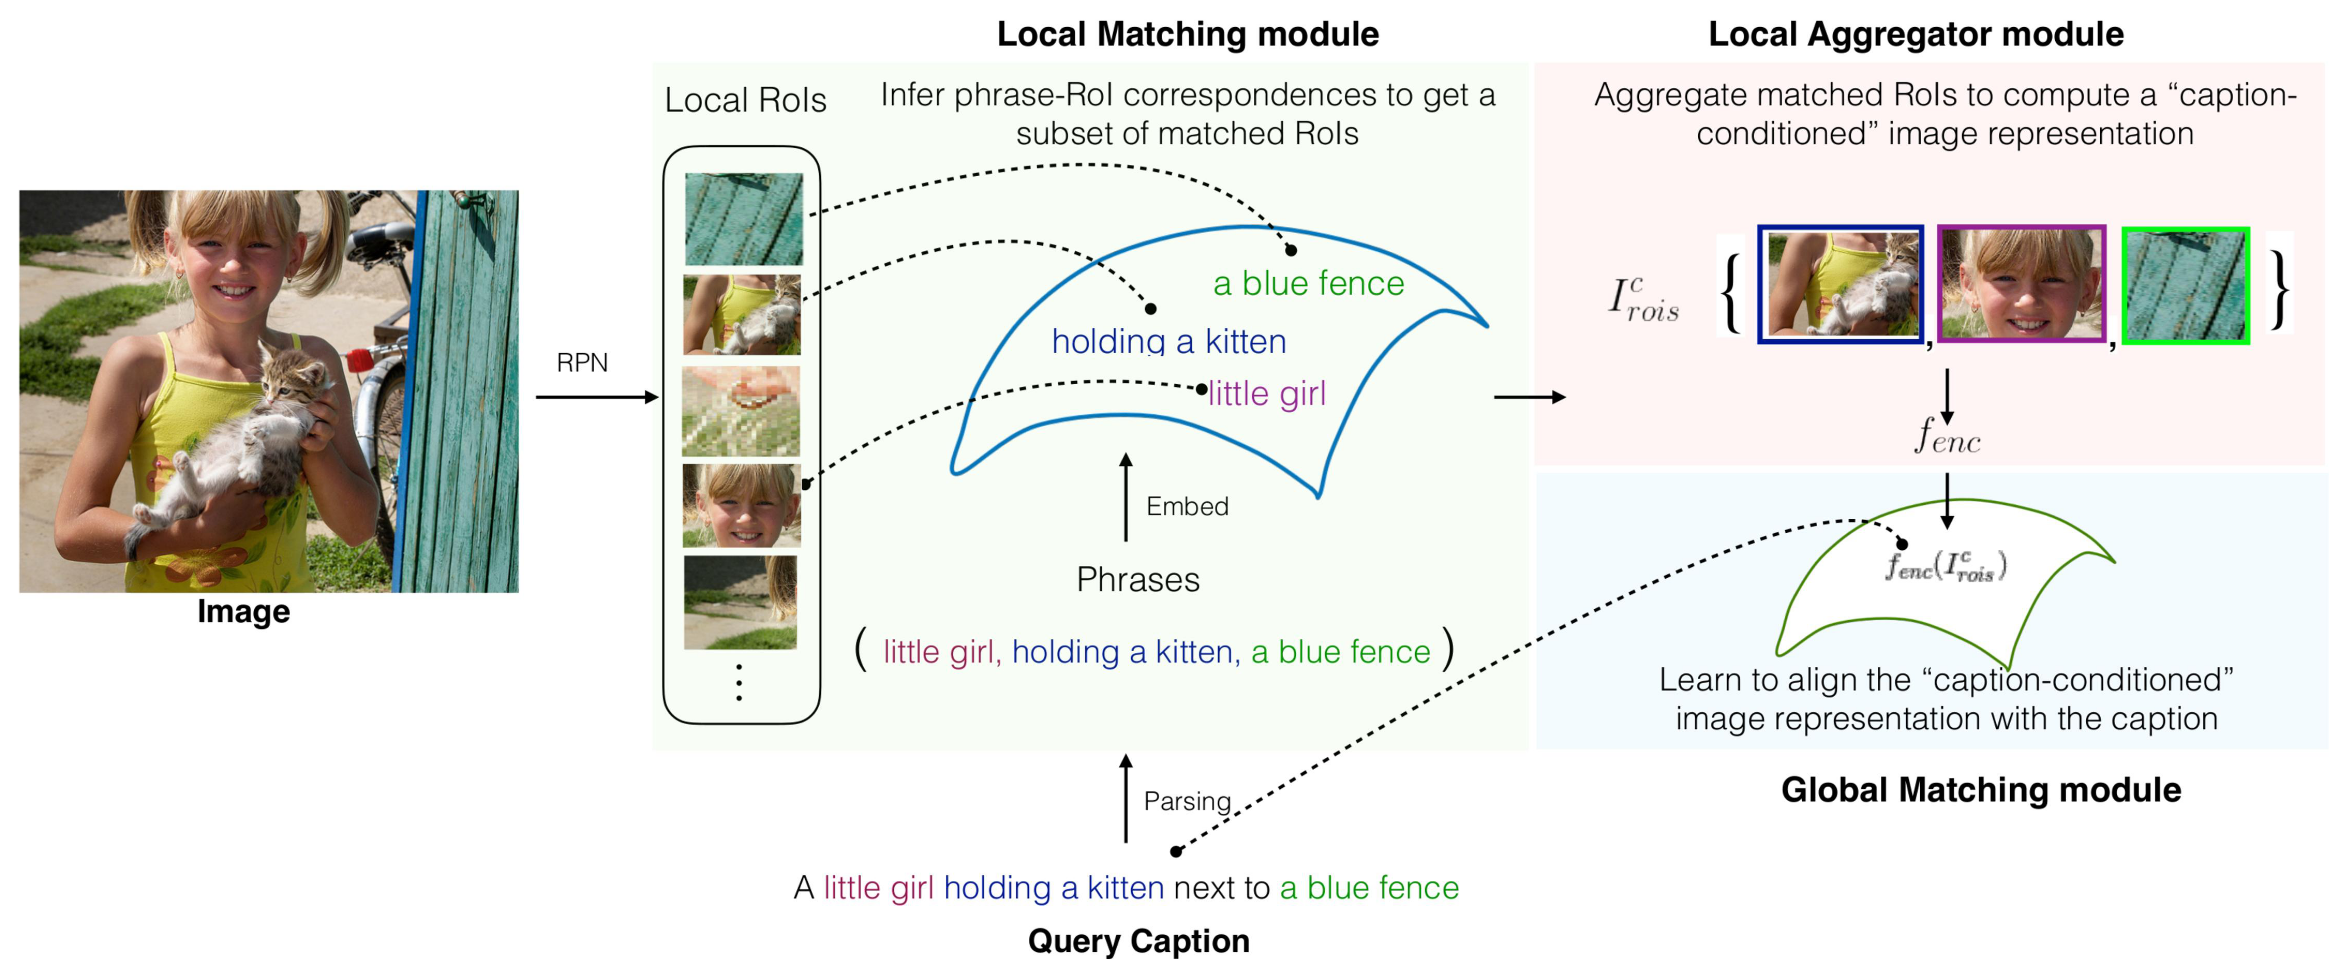
\includegraphics[width=.8\textwidth]{figures/align2ground-model.png}
  \caption[Align2Ground model overview]{Align2Ground model overview
  \cite{datta2019align2ground}. The outputs from a Region Proposal
  Network (RoIs) and the shallow parser (phrases) are fed into the
  Local Matching module which infers the latent phrase-RoI
  correspondences. The Local Aggregator module then digests these
  matched RoIs to create a discriminative, caption-conditioned visual
  representation -- which is then used to align the image-caption
  pairs in the Global Matching module.}
  \label{fig:align2ground-model}
\end{figure}

An important contribution in phrase grounding comes from the work of
J. Wang in \etal{} in \cite{wang2019phrase}. In contrast to other
works which attempt to learn mappings between textual and visual
information from examples of phrase-image region correspondences
(strong supervision) or from phrase-image pairs (weak supervision),
they propose the first method for the phrase localization problem
where neither training procedure nor paired, task-specific data is
required. They argue that such a ``non-paired'' setting better
reflects how humans localize objects in images -- not by memorizing
paired examples, but by assembling prior knowledge from more general
sources and tasks (e.g. recognizing concepts or attributes) to tackle
a more specialized task (phrase localization). As a consequence, their
model has the advantage of being simple and interpretable, acting as a
strong baseline for the novel, non-paired settings. Their model is
built on three steps, as Fig.~\ref{fig:phraseloc-model} shows. In the
first stage, they employ many object detectors (tfcoco, tfcoco2,
places365, yolo9000, colour) that vary in number and type of
categories covered, training data and accuracy in order to explit
their variance and redundancy to retrieve information on objects in
images. Note that use pretrained models for detectors, hence, no
training is performed. The second stage of our model bridges the query
phrase to be localized and the output of detectors. It computes the
semantic similarity between each phrase and the detector concept
labels. The intuition is that the detected instance of a concept that
is very similar or related to a word or phrase in the query is most
likely to be the target object. Similarly to \cite{chen2018knowledge},
they represent queries $q$ and labels $c$ as $300$-dimensional CBOW
word2vec embeddings. The goal of this stage is to compute a ranked
list of candidate bounding box detections based on their similarity to
the aggregate query phrase. Such list is extracted by computing a
similarity function $S(q, c)$ in the word embedding space between the
aggregate emebdding of a query and the embedding of a label. They
explore two approaches to aggregate the words in query phrases: as a
single vector by summing the word vectors and normalizing to unit
vector (w2v-avg), or by representing each word individually (w2v) and
using only one of the words for localization. For the latter, they
select the word with the highest semantic similarity to any detected
concepts (w2v-max). Intuitively, they only consider one word from the
phrase for localization, where this word has the highest similarity to
a detected concept. Alternatively, they can use the last word for
localization (w2v-last), assuming the last word is the head word.
The third an last stage localizes the bounding box given the ranked
list of candidates. The adopted localization approach is to select
from candidate detections the concept most similar to the query
phrase. Where multiple instances of the same concepts are detected,
they experiment with different tie-breaking strate gies:
\begin{enumerate*}[label=(\roman*)] 
  \item selecting a random instance;
  \item selecting the in- stance with the largest bounding box; 
  \item selecting the instance with the highest class prediction
  confidence;
  \item generating a minimal bounding box enclosing all instances
  (union); and
  \item using consensus from detectors. 
\end{enumerate*} 

\begin{figure}
  \centering
  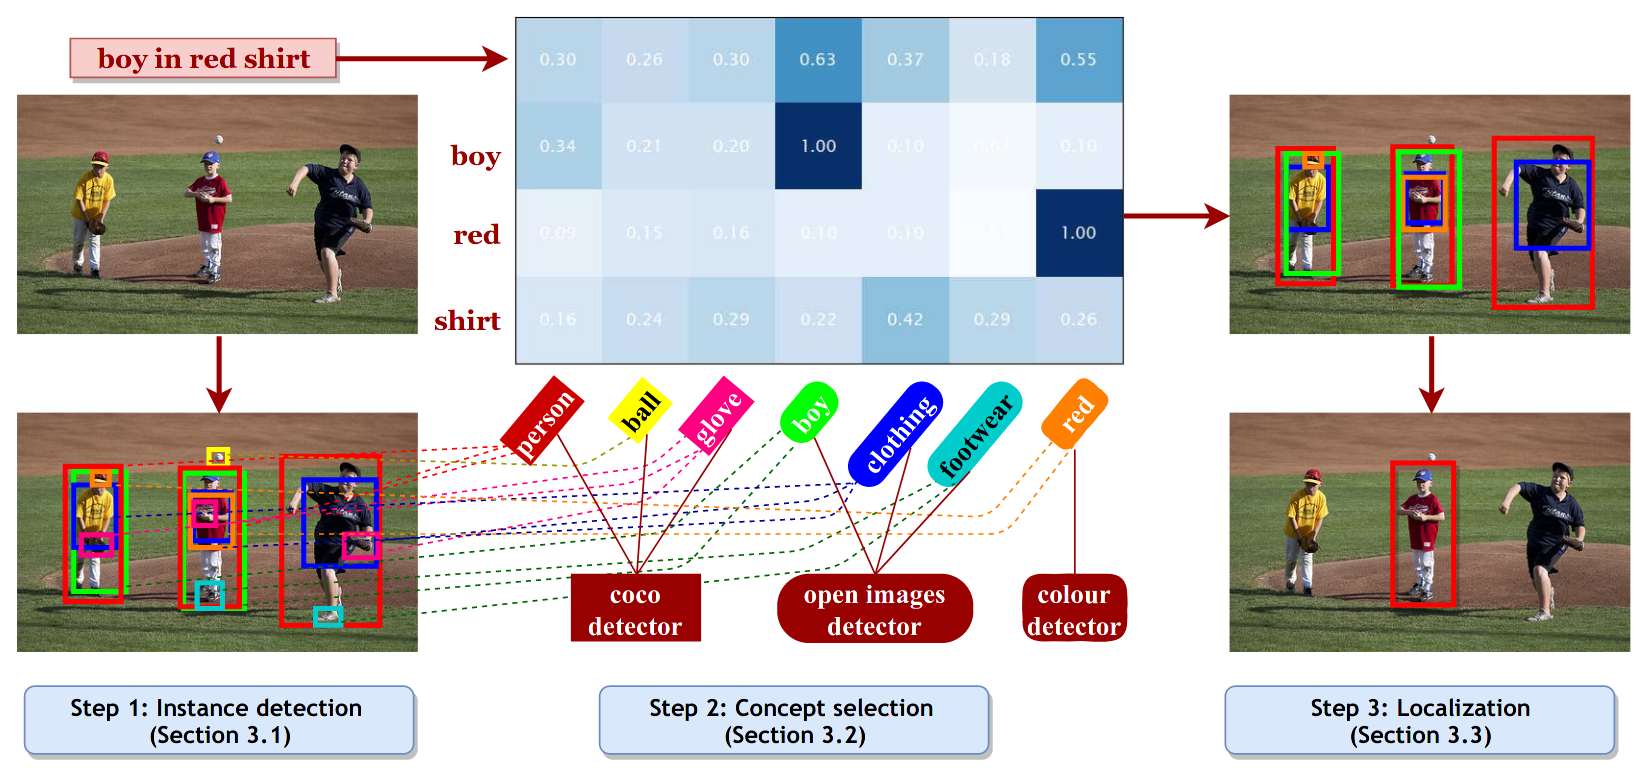
\includegraphics[width=.8\textwidth]{figures/phraseloc-model.png}
  \caption[Phrase Localization without Paired Training Examples
  model overview]{Phrase Localization without Paired Training
  Examples model overview \cite{wang2019phrase}. In the figure is
  depicted the three stages of the proposed model for non-paired
  phrase localization. The instance detection phase detects
  instances of various concepts using pre-trained detectors. The
  concept selection stage ranks these detected concepts against the
  query phrase (using pre-trained word embeddings) and forwards the
  best candidate concept instance(s) to the localization phase,
  where the model predicts the final bounding box for the query
  phrase.}
  \label{fig:phraseloc-model}
\end{figure}

T. Gupta \etal{} in \cite{gupta2020contrastive} showed how to properly
exploit weak annotations. They propose a model that learns phrase
grounding by optimizing word-region attention to maximize a lower
bound on mutual information between images and caption words.
Basically, given pairs of images and captions, they maximize
compatibility of the attention-weighted regions and the words in the
corresponding caption, compared to non-corresponding pairs of images
and captions. The key idea is to construct effective negative captions
for learning through language model guided word substitutions.
Technically, they first extract region and word features using an
object detector and a language model respectively. Contrastive
learning trains a word-region attention mechanism as part of a
compatibility function $\phi_\theta$ between the set of region
features from an image and individual contextualized word
representations. The compatibility function is trained to maximize a
lower bound on mutual information with two losses. For a given caption
word, $\calL_{img}$ learns to produce a higher compatibility for the
true image than a negative image in the mini-batch. $\calL_{lang}$
learns to produce a higher compatibility of an image with a true
caption-word than with a word in a negative caption. They construct
negative captions by substituting a noun word like ``donut'' in the
true caption like ``Chocolate donut in front of a computer'' with
contextually plausible but untrue words like ``cookie'' using a
language model.

Q. Wang \etal{} in \cite{wang2020maf} proposed a multimodal alignment
framework (MAF), outlined in Fig.~\ref{fig:maf-model} that joins the
contrastive learning exploiting weakly-supervised annotations and the
power of external knowledge from pretrained object detector. Inspired
by \cite{wang2019phrase} which encompasses many etherogeneous
categories, they employ the Faster-R CNN
(Sec.~\ref{subsec:faster-rcnn}) object detector trained on $1600$
classes and $400$ attributes. Using a linear projection, they join
proposal features with the word embedding of proposal class label and
proposal attribute label, yielding $\bm{v}_m$. For the textual part,
they embed phrase $\bm{p}_n$ throught word embeddings yielding
$\bm{h}_n,k$ and then, forach $k$-th word in phrase and foreach $n$-th
phrase, they compute a score $\bm{a}^m_{n,k}$ representing the
similarity between such word $\bm{h}_{n,k}$ and proposal features
representation $\bm{v}_m$. The final attention score is the maximum
similarity between proposal features representation and word features
representation. Such attention is the normalized with softmax function
and used as weight for averaging words representation in phrase. A
projection matrix construct the final representation $\bm{e}_n$ for
phrases $p_n$. The model is optimized by a contrastive loss $\calL$
that aims to learn the visual and textual features by maximizing the
similarity score between paired image-caption elements and minimizing
the score between the negative samples:
\begin{equation}
  \calL = - \log \frac{e^{sim(I, S)}}{ \sum_{I' \in batch} e^sim(I', S) },
\end{equation}
where $sim(I, S)$ is the similarity function between image and query
sentence defined as:
\begin{equation}
  sim(I, S) = \frac{1}{N} \sum_n \max_m A_{n,m},
\end{equation}
where $A \in \Rset^{N \times M}$ is the phrase-object similarity
matrix, and its component is computed as:
\begin{equation}
  A_{n,m} = \bm{e}^T_n \bm{v}_m.
\end{equation}
Particularly, for each caption sentence, they use all the images $I′$
in the current batch as candidate (negative) examples.

\begin{figure}
  \centering
  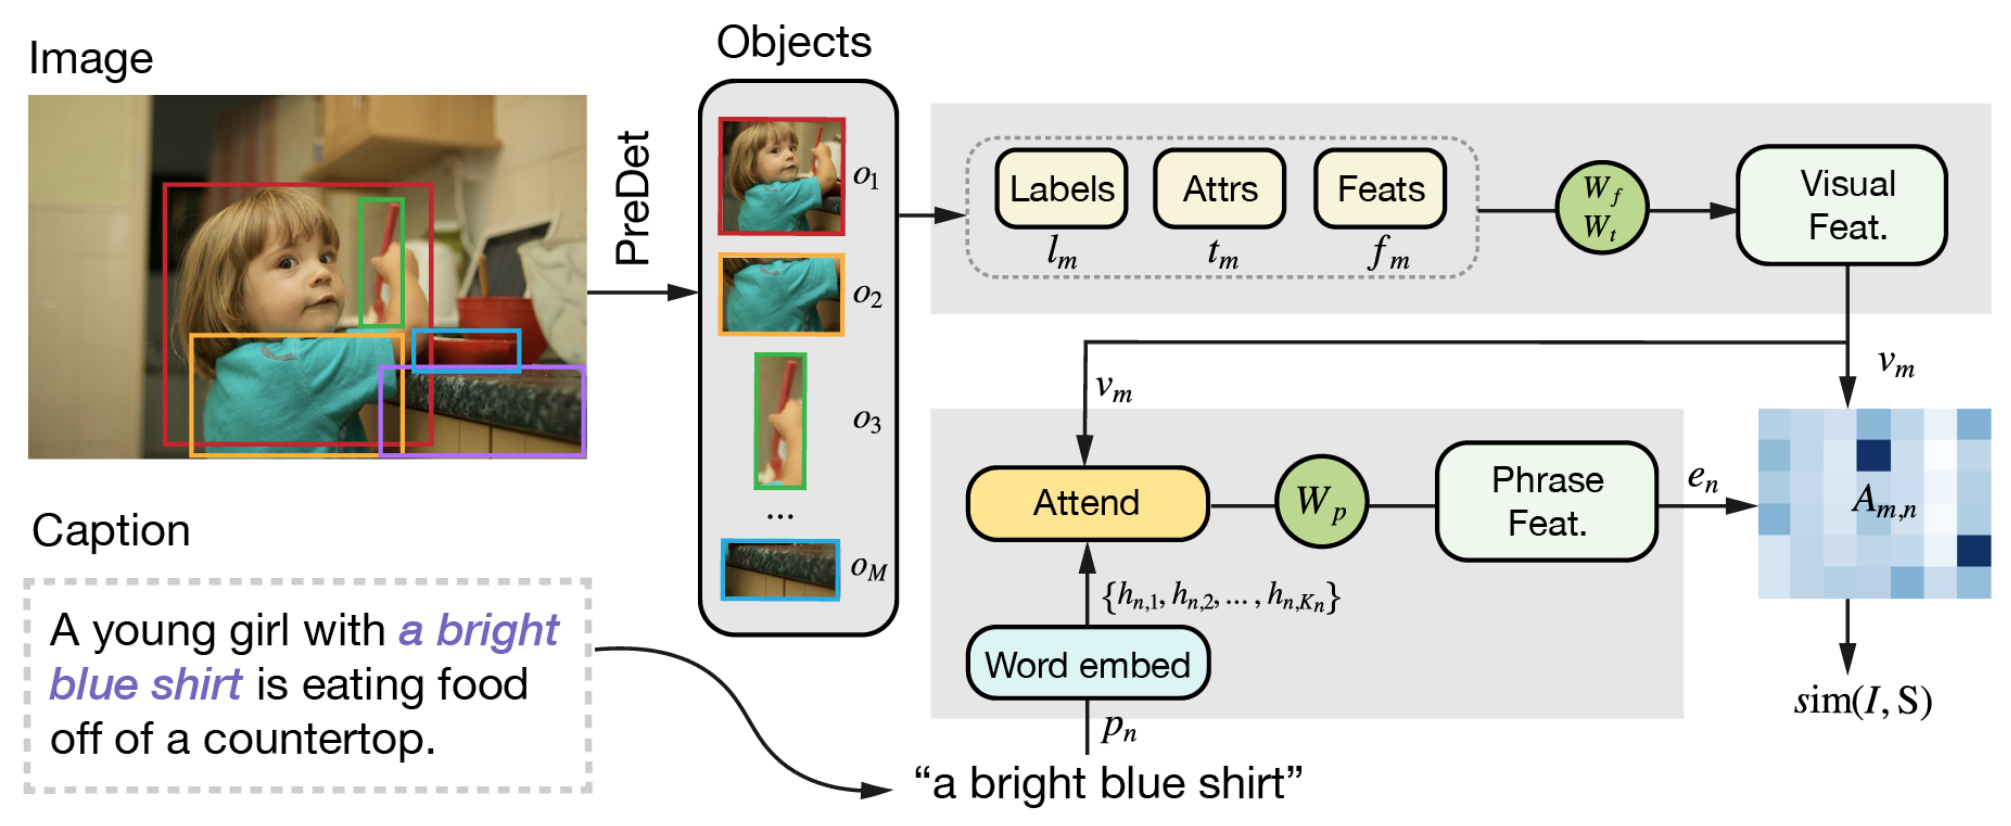
\includegraphics[width=.8\textwidth]{figures/maf-model.png}
  \caption[Multimodal Alignment Framework model overview]{Overview
  of our proposed Multimodal Alignment Framework (MAF)
  \cite{wang2020maf}. A dataset of images and their captions is the
  input to our model. PreDet predicts bounding boxes for objects in
  the image and their labels, attributes, and features, which are
  then integrated into visual feature representations. Attention is
  applied between word embedding and visual representations to
  compute the visually-aware language representations for phrases.
  Finally, a multi-modal similarity function is used to measure the
  caption-image relevance based on the phrase-object similarity
  matrix.}
  \label{fig:maf-model}
\end{figure}

In terms of quantitative evaluation, models developed under supervised
settings show a strong boost in performance. Here, the information of
which is the bounding box that grounds the query is available. During
years, the scientific community devoted much effort solving the phrase
localization problem, leading to the development of different very
different strategies. Z. Yang \etal{} in \cite{yang2019fast} designed
a novel one-stage model (Sec.~\ref{sec:two-stage-vs-one-stage}), whose
goal is to outperform existing propose-and-rank two-stage methods
where the performances are capped by the quality of the region
candidates. ``if none of the candi dates could cover the ground truth
region'', they argue, ``there is no hope in the second stage to rank
the right region to the top''. To avoid this caveat, they propose a
one-stage model that enables end-to-end joint optimization. The main
idea is to fuse text query's embedding into the YOLOv3 object detector
(Sec.~\ref{subsec:yolo}), augmented by spatial features so as to
account for spatial mentions in the query. In \cite{sadhu2019zero}, A.
Sadhu \etal{} on the same line of \cite{yang2019fast} proposed a
one-stage model focusing on the slightly different task of Zero Shot
Grounding, which can include unseen nouns in phrases. They argue that
a two-stage approach (Sec.~\ref{sec:two-stage-vs-one-stage}) is an
obstacle due to the constrained generation of appropriate proposals.
Instead, they propose a single-stage model which combines the detector
network and the grounding system and predicts classification scores
and regression parameters. A completely different approach is adopted
by H. Zhang \etal{} in \cite{zhang2018grounding} where, based on the
variational Bayesian method, they caputeres context's information by
exploiting reciprocal relatiopn between the referent and context. D.
Rigoni \etal{} in \cite{rigoni2021better} proposed a novel loss for
the problem of phrase grounding. They show thay, although using a
simple multi-modal feature fusion component, their model is able to
reach good performance. Such loss employs metrics like Intersection
Over Union (IoU) and Complete IoU (CIoU).

\section{Visual Textual Knowledge Entity Linking}

Visual Textual Knowledge Entity Linking (VTKEL) introduced by S. Dost
\etal{} in \cite{dost2020jointly, dost2020vtkel, dost2020visual}, is a
more complex task than phrase localization: it requires an artificial
agent to jointly recognize the entities shown in the image and
mentioned in the text, and to link them to its prior background
knowledge. The solution to the VTKEL problem could lead to major
scientific advancement towards a better understanding of semantic
information contained in the image and textual sentence, respectively.
In fact, the knowledge graph allows to introduce semantic reasoning on
the information contained in both the image and the textual sentence,
which could lead to innovative solutions for the weakly supervised
phrase localization problem and for the partially annotated dataset
problem.

\section{Visual Question Answering}

Visual Question Answering (VQA) is a computer vision task where a
system is given a text-based question about an image, and it must
infer the answer \cite{kafle2017visual}. Questions can be arbitrary
and can encompass many computer vision task, varying from object
recognition or detection to attribute or scene classification and also
to counting. Beyond this, there are many more complex question that
can be asked, such as questions about spatial relationships among
objects and common sesnse reasoning question. Under this definition,
phrase localization becomes a foundamental building block for VQA
systems.
